\documentclass[11pt]{report} 

\usepackage[a4paper]{geometry}
\usepackage[portuguese]{babel}
\usepackage{hyphenat}
\usepackage{projectreport}
\usepackage{graphicx}
%
\usepackage{minted}
\setminted[bash]{
    frame=lines,
    breaklines,
    fontsize=\footnotesize,
    framesep=2mm
}
\setminted[python]{
    frame=lines,
    breaklines,
    fontsize=\footnotesize,
    framesep=2mm
}
\usepackage{hyperref}
\usepackage{subfiles}
\usepackage{lscape}

% Used for displaying a sample figure. If possible, figure files should
% be included in EPS format.
%
% If you use the hyperref package, please uncomment the following line
% to display URLs in blue roman font according to Springer's eBook style:
% \renewcommand\UrlFont{\color{blue}\rmfamily}

\newcommand{\name}{Marco Sousa $(62608)$, José Malheiro $(93271)$ e Miguel Fernandes $(94269)$}
\newcommand{\course}{Licenciatura em Engenharia Informática}
\newcommand{\projecttitle}{Conceção de Compiladores - \textit{Pandoc}}
\newcommand{\submissiondate}{Maio 2022}

\begin{document}

\maketitle    

\tableofcontents

\pagenumbering{arabic}

% \begin{abstract}
% \keywords{Expressões regulares \and Python \and Templates \and Gramática Independente de Contexto \and Compiladores.}
% \end{abstract}
%
%
%
\chapter{Introdução}
\section{Contextualização} 

\subfile{intro/context.tex}

\section{Breve Descrição do Trabalho Proposto}

\subfile{intro/descr.tex}

\chapter{\textit{HandleDoc}}
O desenvolvimento do \textit{software} apresentado neste relatório,
remete-se à utilização de um paradigma de programação orientada aos objetos.
Procurou-se, ao longo da sua modelação, realizar uma descentralização de responsabilidades,
através da utilização da hierarquia de classes e da geração de classes especializadas que
derivam de outras abstratas, permitindo a unificação do sistema.

Assim, por forma a estruturar a solução, começou por se modular uma gramática abstrata.
Posteriormente, identificou-se as palavras reservadas que a definiam.
Por último, adicionou-se os vários símbolos terminais e literais que permitiam
compôr a sintaxe de \textit{templating}.

A partir da gramática abstrata, foi possível construir um diagrama de classes
correspondente à representação da árvore de sintaxe concreta.

Irá apresentar-se a gramática independente de contexto, em particular os sínbolos não terminais,
seguido do analisador léxico e, por fim, o \textit{parser}.

\section{Gramática Independente de Contexto} \label{subsec:grammar}
\subfile{hdoc/gic.tex}

\section{Analisador Léxico} \label{subsec:lex}
\subfile{hdoc/state.tex}

\section{\textit{Parser}} \label{subsec:strat}
\subfile{hdoc/strategy.tex}


\section{\textit{HandleDoc}}
\subsection{Manual}
\inputminted{bash}{../assets/manual.txt}

\subsection{Funcionalidades Compactadas}
\subfile{hdoc/func_table.tex}


\chapter{Conclusões}

\subfile{conclusion/conc.tex}

\chapter{Anexos}\label{sec:anexos}

\section{Gramática} \label{fig:grammar}
\inputminted{bash}{assets/gramatica.txt}

\section{Diagrama de Máquina de Estados}
\begin{figure}[!ht]
    \centering
    \includegraphics[width=\linewidth]{assets/Máquina_estados.png}
\end{figure}

\section{Diagrama de Classes} \label{sec:classes}
\begin{landscape}
    \centering
    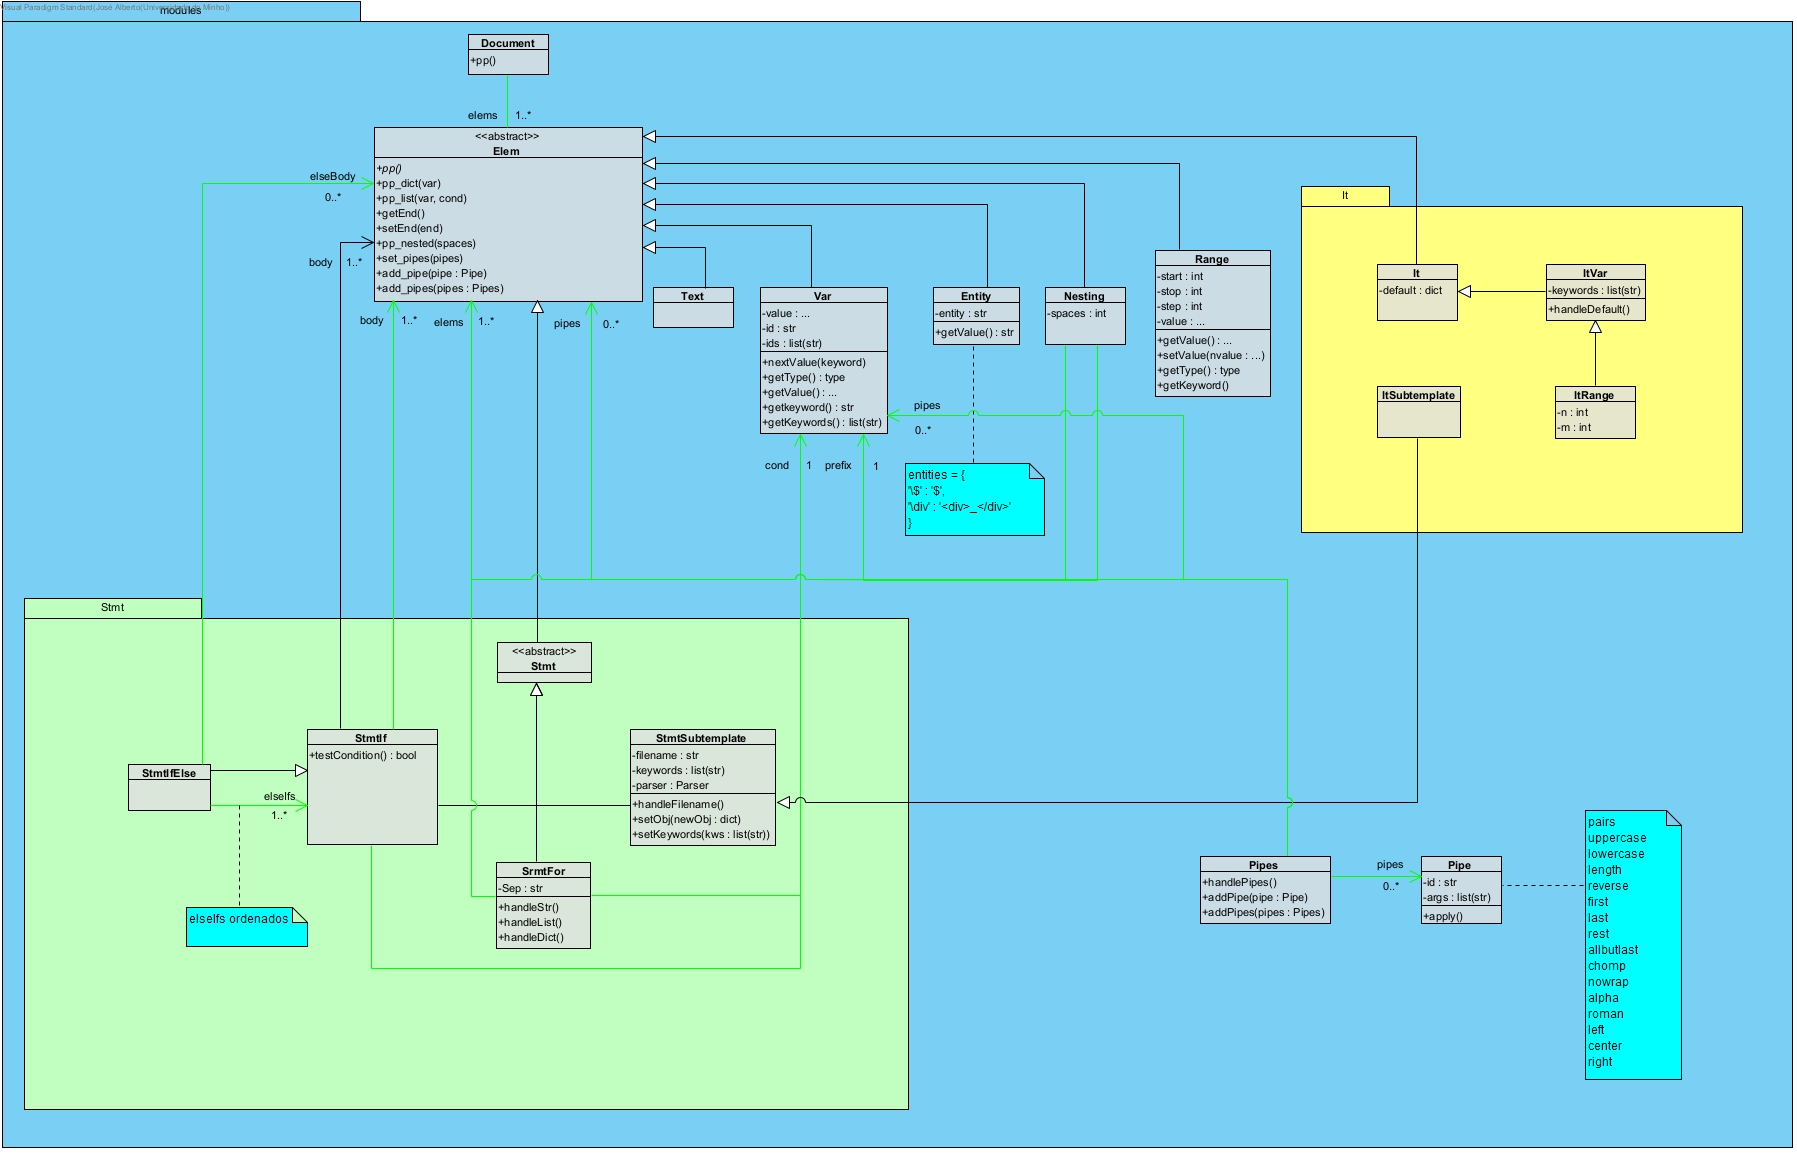
\includegraphics[width=\linewidth]{assets/class_diagram.jpg}
\end{landscape}
%
% ---- Bibliography ----
%
% BibTeX users should specify bibliography style 'splncs04'.
% References will then be sorted and formatted in the correct style.
%
% \bibliographystyle{splncs04}
% \bibliography{mybibliography}
% %
% \begin{thebibliography}{1}
% \bibitem{ref_article1}
% Author, F.: Article title. Journal \textbf{2}(5), 99--110 (2016)

% \bibitem{ref_lncs1}
% Author, F., Author, S.: Title of a proceedings paper. In: Editor,
% F., Editor, S. (eds.) CONFERENCE 2016, LNCS, vol. 9999, pp. 1--13.
% Springer, Heidelberg (2016). \doi{10.10007/1234567890}

% \end{thebibliography}

\end{document}